\chapter*{10.08. --- Cywilizacja po raz drugi, ostatni}

Początek dnia można streścić krótko --- długie spanie, późne śniadanie, późny wyjazd. Ot, taki typowy niedzielny poranek, kiedy to wszystko się odbywa dość sennie\textellipsis Dlatego aż przecieraliśmy oczy ze zdumienia, gdy o 11:00 zobaczyliśmy, jak ,,naszą'' miedzą sunie ku nam olbrzymi traktor. \emph{,,Pewnie zaraz skręci gdzieś w bok''} ---- myślimy sobie. Ale nie, on jedzie dalej prosto na nas. Gdy maszyna znalazła się wreszcie w odległości ledwie stu metrów od nas, rzuciliśmy się do gorączkowego pakowania rzeczy i zwijania namiotów. Bo a nuż gospodarz będzie chciał nas pogodnić widłami\textellipsis albo traktorem? Nic z tych rzeczy! Kierowcą traktora okazał się sympatyczny Pan Islandczyk, który sprawiał wrażenie rozbawionego całą sytuacją. Płynną angielszczyzną zaczął podpytywać skąd jesteśmy i jak nam się udała wyprawa, spokojnie poczekał aż przestawimy namioty i w ogóle tylko brakowało, by zaprosił nas na obiad do siebie.

Po tych porannych przygodach ruszyliśmy sprawnie do Akureyri, by jak najwcześniej zajechać do świątyni konsumpcji i mekki wszystkich islandzkich turystów --- do Bonusa!

\hint{Plan Akuyreri można dostać na stacjach benzynowych (jedna z~nich znajduje się tuż za groblą). Bonus znajduje się przy \road{1} na północy miasta, nie trzeba krążyć.}

W Bonusie zakupiliśmy liczne dobra luksusowe: salami, czekoladę, ananasy, masło, jogurty\textellipsis Z części z nich przyrządziliśmy niezwłocznie, od razu na miejscu, extra paszę de luxe w ilości ,,do porzygu''. Głodni byliśmy, to nikt sobie nie krzywdował, w efekcie czego chwilę później ledwo-ledwo udawało nam się wtaczoczyć na pagórki przy wylocie z miasta!

%TODO: zrobić z tego środowisko
%\img{./photos/x-s-2014-08-10_13-54-57__90.jpg}{feeder_de_luxe}{Pasza de luxe --- na jogurcie, z bananem\textellipsis}

\begin{figure}[h]
	\centering
	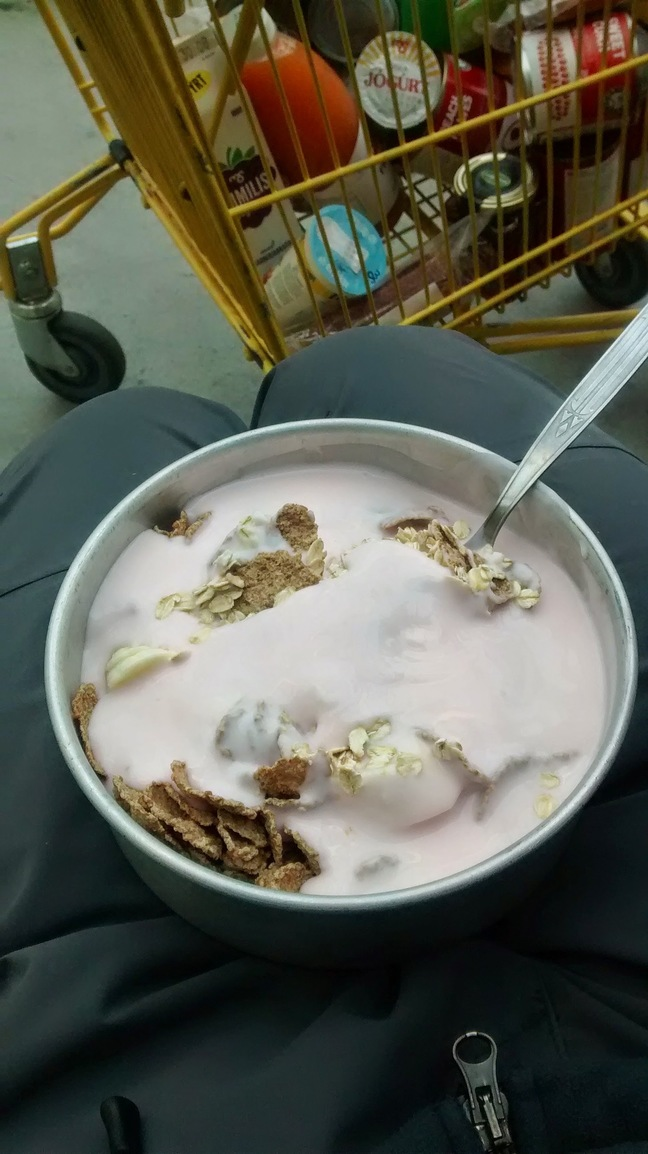
\includegraphics[height=.7\linewidth]{./photos/x-s-2014-08-10_13-54-57__90.jpg}
	\caption*{Pasza de luxe --- na jogurcie, z bananem\textellipsis}
	\label{img:feeder_de_luxe}
\end{figure}

Dzisiejsza droga jest jak ze snu: ładne, równe doliny, długie podjazdy i konkretne zjazdy\footnote{Lepiej pokonywać tę trasę od strony Akureyri, bo wtedy na zjazdach nie ma serpentyn!} --- żadnego jeżdżenia po pagórkach! Szkoda tylko, że panuje aż tak duże natężenie ruchu --- zupełnie, jak na polskich drogach wojewódzkich. Dobitnym dowodem tego, że droga nie była trudna niech będzie fakt, że w połowie zjazdu zatrzymaliśmy się na kanapki (z~masłem i salami --- mniam!). Warto zaznaczyć, że po raz pierwszy (chyba?) tak pojedliśmy w~południe koło Bonusa, że na dobrą sprawę kanapki i ciastka jedliśmy w drodze bardziej z łakomstwa niż z rzeczywistej potrzeby zasypania organizmu kolejną porcją kalorii!

Na zjeździe z przełęczy po raz trzeci widzę tych samych wrocławian (dwa samochody na blachach DW) --- wcześniej mijali mnie na \road{85} i podczas tego zjazdu, kiedy to podziwialiśmy zachód słońca. Ot, uroki jeżdżenia po Islandii, gdzie właściwie wszyscy poruszają się po tej samej drodze i oglądają te same miejsca! Pozostali znajomi coś nie pokazują się: Holendrów brak, Pani Polki (raczej) już nie spotkamy (bo nie zamierzała robić \road{F35}), a Pan Rusek objeżdża Islandię w przeciwnym kierunku.

Zmiany pogody w górskich regionach Islandii zaskakują --- z doliny gdzie niebo zasnute było szczelnie gęstymi chmurami zjeżdżamy prosto do kolejnej, gdzie z kolei praży ostre słońce. Fakt, że ,,deszczu niet'' i że wiatr (wyjątkowo) nie wieje w twarz upoważnia nas do określenia całości mianem ,,naprawdę pięknej islandzkiej pogody''! Lecz czymże byłaby podróż bez przygód? Ostatnie 15~km potwornie męczymy, bo jednak wiatr odkręcił. Wieje tak mocno, że na tym krótkim odcinku musieliśmy zrobić jeszcze jeden odpoczynek --- autentycznie potrzebowaliśmy nabrać sił do dalszej walki z wiatrem!

W Varmahlíð mieliśmy do wyboru dwa kempingi --- jeden tuż przy wjeździe, drugi ponad kilometr dalej. Choć generalnie nogi nam już z tyłka wychodziły, zdobyliśmy się na ten ostatni wysiłek, a to z bardzo prostej przyczyny --- średnią mieliśmy ochotę, by przy którymś podmuchu wiatru nasze namioty odleciały. Tak, pod tym względem Kempingu Tjödum i Skagarfirði był zdecydowanie faworytem --- zaciszny, położony wśród drzew, zrobiony na wzór europejski (a więc: boksy na namioty bądź samochody wytyczone szpalerami drzew). Za przyzwoitą cenę (1100~kr od osoby, 100~kr za namiot i jeszcze 250~kr za prysznic) otrzymuje się dostęp do ciepłej łazienki, która od biedy może robić za kuchnię, oraz grzejące na maks liczne kaloryfery. Wreszcie robiąc pranie można mieć pewność, że na rano będzie ono suche!

Po raz pierwszy widzimy na Islandii księżyc! Bynajmniej nie dlatego, że chodzimy spać z kurami --- po prostu po raz pierwszy wieczorem na niebie niemal nie ma chmur!
